\documentclass[architecture]{compas2018}
%%%%%%%%%%%%%%%%%%%%%%%%%%%%%%%%%%%%%%%%%%%%%%%%%%%%%%%%%%%%%%%%%%%%%

\toappear{1} % Conserver cette ligne pour la version finale

\usepackage{tikz}
\tikzset{
  hwblock/.style={draw, rectangle, rounded corners=.3, very thick, fill=black!5, font=\sf, minimum height=5ex},
  hwbus/.style={very thick,>=stealth},
  hwwire/.style={thin, >=stealth, },
  hwword/.style={draw, rectangle, minimum height=3ex},
  bitwidth/.style={font=\scriptsize,midway,right}
}

\newcommand{\reg}{\textit{reg}}
\newcommand{\const}{\textit{const}}
\newcommand{\shiftval}{\textit{shiftval}}
\newcommand{\cond}{\textit{cond}}
\newcommand{\ctr}{\textit{ctr}}
\newcommand{\size}{\textit{size}}
\newcommand{\addr}{\textit{addr}}

\begin{document}

\title{Une architecture minimisant les échanges\\ entre processeur et mémoire}

\author{Florent de Dinechin, \\Sébastien Michelland, Maxime Darrin, Antonin Dudermel, Alban Reynaud}

\address{
  % \begin{tabular}{cc}
  %   ENS-Lyon & INSA Lyon \\
  %   \texttt{nom.prenom@ens-lyon.org} \\
  % \end{tabular}
}

\date{\today}

\maketitle

\begin{abstract}
Dans une architecture de von Neumann, le processeur communique avec la mémoire au moyen d'un bus d'adresses et d'un bus de données de grandes tailles (entre 16 et 64 bits).
C'est une contrainte pour l'encodage des instructions du processeur, comme le montre un survol historique des jeux d'instruction dominants.
Or les échanges de données représentent le gros de l'énergie dépensée.
Cet article fait l'exercice de lever cette contrainte, dans le but de minimiser le nombre de bits échangés entre le processeur et la mémoire.
Il décrit une architecture 64 bits dont la mémoire est adressable par bit, avec un seul signal de données entre le processeur et la mémoire.
Ceci permet d'avoir des instructions de taille arbitraire.
Pour ne pas devoir envoyer une adresse complète à la mémoire à chaque accès, la solution proposée est l'usage de pointeurs auto-incrémentés dupliqués dans la mémoire et le processeur.

Cet article décrit aussi une expérience pédagogique réalisée à l'ENS-Lyon (ce qui explique en partie certains choix simplistes).
Un premier jeu d'instruction a été défini en TD et son encodage choisi à la main.
Ceci a permis aux étudiants d'écrire en binôme un assembleur et un simulateur, puis plusieurs milliers de lignes de programmes allant du petit noyau de calcul au jeu vidéo et à l'émulateur.
Sur les traces de ces programmes, on a pu ensuite calculer un encodage optimal des instructions des instructions en fonction de leur fréquence via des arbres de Huffmann, et les comparer à l'encodage initial.
On arrive à une taille moyenne d'instruction entre 9 et 15 bits suivants les programmes.
 Ces expérimentations montrent aussi que le code représente une part importante des données transitant entre processeur et mémoire. 
 L'article discute enfin les limites de cette approche, et d'éventuelles solutions pour y remédier.
\end{abstract}

%=========================================================
\section{Introduction et motivation}
%=========================================================


\section{Présentation du jeu d'instruction}
\subsection{Registres généralistes}
Dans cette expérience nous avons fixé le nombre de registres à 8.
C'est un choix arbitraire et discutable, motivé par des raisons pédagogiques (rencontrer cette limite dès l'écriture de programmes simples) et par une raison pratique (encoder le numéro de registre sur aussi peu de bits que possible).

Les registres généralistes sont notés r0 à r7.
Ils sont tous parfaitement identiques, sauf r7 qui reçoit l'adresse de retour en cas de \texttt{call}.

\paragraph{Autocritique} Les architectures modernes offrent typiquement entre 16 et 64 registres.
Elles offrent également des mécanismes qui exposent dans le jeu d'instruction un sous-ensemble des registres architecturaux, soit de manière explicite (les fenêtres de registres du SPARC), soit de manière implicite (le techniques de renommage qui permettent l'exécution superscalaire).

On pourrait avoir un nombre de registres beaucoup plus grand avec un encodage compact des registres les plus utilisés.

\subsection{Format général des mnémoniques}
Les instructions commencent toutes par un mnémonique, suivi des opérandes, le tout séparé par des espaces.

Les instructions ALU viennent en version 2 et 3 opérandes, la destination venant toujours en premier.
Par exemple, \\
 \begin{tabular}{lcl}
 \texttt{add2 r0 r1}&& réalise $r_0 \leftarrow r_0+r_1$. \\
 \texttt{add3 r0 r1 r2}&& réalise $r_0 \leftarrow r_1+r_2$.
 \end{tabular}
 
Le suffixe \texttt{i} signifie que le dernier opérande est une constante immédiate, par exemple:\\
 \begin{tabular}{lcl}
 \texttt{add2 r0 1}&& réalise $r_0 \leftarrow r_0+1$. \\
 \end{tabular}

L'assemblage commence à l'adresse 0, qui est celle à laquelle notre processeur démarre.

 
Sucre syntaxique offert par l'assembleur:
\begin{itemize}
\item On peut utiliser des labels pour les sauts.
\item Le mot-clé \texttt{.const n xxxx}  réserve $n$ bits de mémoire, initialisés à la constante xxxx, qui est priée de tenir sur $n$ bits.
\item Les constante hexadécimales sont préfixées par \texttt{0x}, par exemple \texttt{0xff}
\item Le commentaire est introduit par un point-virgule \texttt{;}
\end{itemize}
 

Exemple de programme :
\begin{verbatim}
  let r0 17     ; l'assembleur va calculer combien de bits il faut pour 17
boucle:	
  sub2i r0 1    ; encodé en 9 bits, et ceci est un commentaire
  jumpif nz boucle  ; encodé en 16 bits, signifie  jump -25 
\end{verbatim}

\subsection{Le jeu d'instructions et son encodage minimal}



La table \ref{tab:opcodes} décrit l'opcode qui commence chaque instruction.

Remarques en vrac: 
\begin{itemize}
\item le not logique est implémenté par xor -1
\item la direction du shift est encodée dans un bit après l'instruction pour économiser un opcode. On aurait pu définir deux opcodes comme pour \texttt{uread}/\texttt{sread} mais c'est plus rigolo de lire \texttt{shift left r1 1}.
\end{itemize}


\begin{table}[!h]
  \caption{Liste des instructions.}
  \label{tab:opcodes}
  Le codage de Huffmann des instructions est basée sur les statistiques des années précédentes.
  Les opérandes d'une instruction la suivent en mémoire. Ils sont encodés comme suit:
  \begin{itemize}
\item \textit{reg} $\in \{\mathtt{r0}, \mathtt{r1}, ..., \mathtt{r7}\}$ et est encodé par le numéro du registre en binaire.
\item \textit{const}, \textit{shiftval} et \textit{addr} sont définis par la table \ref{tab:constantes}. La dernière colonne de la table  \ref{tab:opcodes} précise si une constante est étendue avec son signe (s) ou des zéros (z).   
\item  \textit{cond} est défini par la table~\ref{tab:conditions}.
\item \ctr\ est défini par la table~\ref{tab:counters}.
\item \textit{dir} peut être le mnemnonique \texttt{left}, encodé par 0, ou le mnemonique \texttt{right}, encodé par 1.
\end{itemize}
\begin{center}
  \begin{tabular}{|l|l|l|l|l|c|}
    \hline  
    opcode  & mnemonic        & operands                      & description                                          & ext. & {MàJ flags} \\
    \hline  
    \hline  
    0000    & \texttt{add2}   & \reg\ \reg\                   & addition                                             &      & zcvn        \\
    \hline
    0001    & \texttt{add2i}  & \reg\ \const\                 & add immediate constant                               & z    & zcvn        \\
    \hline
    0010    & \texttt{sub2}   & \reg\ \reg\                   & subtraction                                          &      & zcvn        \\
    \hline
    0011    & \texttt{sub2i}  & \reg\ \const\                 & subtract immediate constant                          & z    & zcvn        \\
    \hline
    0100    & \texttt{cmp}    & \reg\ \reg\                   & comparison                                           &      & zcvn        \\
    \hline
    0101    & \texttt{cmpi}   & \reg\ \const\                 & comparison with immediate constant                   & s    & zcvn        \\
    \hline
    0110    & \texttt{let}    & \reg\ \reg\                   & register copy                                        &      &             \\
    \hline
    0111    & \texttt{leti}   & \reg\ \const\                 & fill register with constant                          & s    &             \\
    \hline
    1000    & \texttt{shift}  & \textit{dir} \reg\ \shiftval\ & logical shift                                        &      & zcn         \\
    \hline
    10010   & \texttt{readze} & \ctr\ \size\ \reg\            & read \size\ memory bits (zero-extended) to \reg\     &      &             \\
    10011   & \texttt{readse} & \ctr\ \size\ \reg\            & read \size\ memory bits (sign-extended) to \reg\     &      &             \\
    \hline
    1010    & \texttt{jump}   & \addr\                        & relative jump                                        &      &             \\
    \hline
    1011    & \texttt{jumpif} & \cond\ \addr\                 & conditional relative jump                            &      &             \\
    \hline
    110000  & \texttt{or2}    & \reg\ \reg\                   & logical bitwise or                                   &      & zcn         \\
    \hline
    110001  & \texttt{or2i}   & \reg\ \const\                 & logical bitwise or                                   & {z}  & zcn         \\
    \hline
    110010  & \texttt{and2}   & \reg\ \reg\                   & logical bitwise and                                  &      & zcn         \\
    \hline
    110011  & \texttt{and2i}  & \reg\ \const\                 & logical bitwise and                                  & {z}  & zcn         \\
    \hline
    110100  & \texttt{write}  & \ctr\ \size\ \reg\            & write the lower \size\ bits of \reg\ to mem          &      &             \\
    \hline
    110101  & \texttt{call}   & \addr\                        & sub-routine call                                     & s    &             \\
    \hline
    110110  & \texttt{setctr} & \ctr\ \reg\                   & store \reg\ to a counter                             &      &             \\
    \hline
    110111  & \texttt{getctr} & \ctr\ \reg\                   & copy the current value of a counter to \reg\         &      &             \\
    \hline
    1110000 & \texttt{push}   & \reg\                         & push value of register on stack                      &      &             \\
    \hline
    1110001 & \texttt{return} &                               & return from subroutine                               &      &             \\
    \hline
    1110010 & \texttt{add3}   & \reg\ \reg\ \reg\             &                                                      &      & zcvn        \\
    \hline
    1110011 & \texttt{add3i}  & \reg\ \reg\ \const\           &                                                      & z    & zcvn        \\
    \hline
    1110100 & \texttt{sub3}   & \reg\ \reg\ \reg\             &                                                      &      & zcvn        \\
    \hline
    1110101 & \texttt{sub3i}  & \reg\ \reg\ \const\           &                                                      & z    & zcvn        \\
    \hline
    1110110 & \texttt{and3}   & \reg\  \reg\ \reg\            &                                                      &      & zcn         \\
    \hline
    1110111 & \texttt{and3i}  & \reg\ \reg\ \const\           &                                                      & {z}  & zcn         \\
    \hline
    1111000 & \texttt{or3}    & \reg\ \reg\ \reg\             &                                                      &      & zcn         \\
    \hline
    1111001 & \texttt{or3i}   & \reg\ \reg\ \const\           &                                                      & {z}  & zcn         \\
    \hline
    1111010 & \texttt{xor3}   & \reg\ \reg\ \reg\             &                                                      &      & zcn         \\
    \hline
    1111011 & \texttt{xor3i}  & \reg\ \reg\ \const\           &                                                      & {z}  & zcn         \\
    \hline
    1111100 & \texttt{asr3}   & \reg\  \reg\ \shiftval\       &                                                      &      & zcn         \\
    \hline
    1111101 & \texttt{}       &                               & reserved                                             &      &             \\
    \hline
    1111110 & \texttt{}       &                               & reserved                                             &      &             \\
    \hline
    1111111 & \texttt{}       &                               & reserved                                             &      &             \\
    \hline
  \end{tabular}
\end{center}
\end{table}


\begin{table}
  \label{tab:constantes}
  \centering
  \caption{Encodage des constantes}
  \begin{tabular}{|l|l|}
    \hline
    \multicolumn{2}{|c|}{\textit{addr} : Encodage \emph{prefix-free} des adresses et déplacements} \\
    \hline
    0 + 8 bits    & adresse ou déplacement sur 8 bits                                              \\
    \hline
    10 + 16 bits  &                                                                                \\
    \hline
    110 + 32 bits &                                                                                \\
    \hline
    111 + 64 bits &                                                                                \\
    \hline
    \hline
    \multicolumn{2}{|c|}{\textit{shiftval} : Encodage \emph{prefix-free} des constantes de shift}  \\
    \hline
    0 + 6 bits    & constante entre 0 et 63                                                        \\
    \hline
    1             & constante 1                                                                    \\
    \hline
    \hline
    \multicolumn{2}{|c|}{\textit{const} : Encodage \emph{prefix-free} des constantes ALU}          \\
    \hline
    0 + 1 bit     & constante 0 ou 1                                                               \\
    \hline
    10 + 8 bits   & octet                                                                          \\
    \hline
    110 + 32 bits &                                                                                \\
    \hline
    111 + 64 bits &                                                                                \\
    \hline
    \hline
    \multicolumn{2}{|c|}{\textit{size} : Encodage \emph{prefix-free} des tailles mémoire}          \\
    \hline
    00            & 1 bit                                                                          \\
    \hline
    01            & 4 bits                                                                         \\
    \hline
    100           & 8 bits                                                                         \\
    \hline
    101           & 16 bits                                                                        \\
    \hline
    110           & 32 bits                                                                        \\
    \hline
    111           & 64 bits                                                                        \\
    \hline
  \end{tabular}
\end{table}



\subsection{Les instructions de branchement }
\label{sec:jumpcallret}

Soit $a$ l'adresse du premier bit suivant l'instruction \texttt{jump} ou \texttt{call} (i.e. la valeur du PC lorsqu'il a fini de lire l'instruction et ses opérandes).
Soit $d$ la valeur de déplacement (encodée dans une constante de type \textit{addr}, et signée).

L'instruction \texttt{jump} réalise $\mathtt{pc}\leftarrow a + c$.
L'instruction \texttt{jumpif} aussi, mais seulement si la condition est vraie.

La condition  est encodée sur trois bits  selon la table~\ref{tab:conditions}.
\newcommand{\bool}{\mathbb{B}}
\newcommand{\booland}{\wedge}
\newcommand{\boolor}{\vee}
\newcommand{\boolnot}[1]{\overline{#1}}
\begin{table} 
  \caption{Condition codes}
  \label{tab:conditions}
\begin{center}
  \begin{tabular}{|c|c|c||l||l|c|}
    \hline  
      &   &   & mnemonic                  & description (after \texttt{cmp} op1 op2)           & {implem.}                                                                           \\
    \hline  
    \hline  
    0 & 0 & 0 & \texttt{eq}, \texttt{z}   & equal, op1 $=$ op2                                 & $z$                                                                                 \\
    \hline
    0 & 0 & 1 & \texttt{neq}, \texttt{nz} & not equal, op1 $\neq$ op2                          & $\boolnot{z}$                                                                       \\
    \hline
    0 & 1 & 0 & \texttt{sgt}              & signed greater than, op1 $>$ op2, two's complement & $\boolnot{z} \booland (n \booland {v}) \boolor (\boolnot{n} \booland \boolnot{v}) $ \\
    \hline
    0 & 1 & 1 & \texttt{slt}              & signed smaller than, op1 $<$ op2, two's complement & $(n \booland \boolnot{v}) \boolor (\boolnot{n} \booland v) $                        \\
    \hline
    1 & 0 & 0 & \texttt{gt}               & op1 $>$ op2, unsigned                              & $\boolnot{z} \booland \boolnot{c}$                                                  \\
    \hline
    1 & 0 & 1 & \texttt{ge}, \texttt{nc}  & op1 $\ge$ op2, unsigned                            & $\boolnot{c}$                                                                       \\
    \hline
    1 & 1 & 0 & \texttt{lt}, \texttt{c}   & op1 $<$ op2, unsigned                              & $c$                                                                                 \\
    \hline
    1 & 1 & 1 & {\texttt{v}}              & {two's complement overflow}                        & {$v$}                                                                               \\
    \hline
  \end{tabular}
\end{center}
\end{table} 

La différence entre \texttt{sgt} et \texttt{gt} s'observe par exemple sur la comparaison entre \texttt{r0} et -1.

L'instruction \texttt{call} copie $\texttt{a}$ dans $r_{7}$, puis réalise $\mathtt{pc} \leftarrow \texttt{d}$
(c'est un peu bizarre de sauter à des adresses négatives mais du coup \emph{addr} est toujours signé).

L'instruction \texttt{return} copie \texttt{r7} dans \texttt{pc}.

\subsection{Les instructions d'accès mémoire}
\label{sec:mem}

\begin{figure}[h]
  \caption{Overview of the processor-memory interface}
  \label{fig:overview}
    \begin{center}
  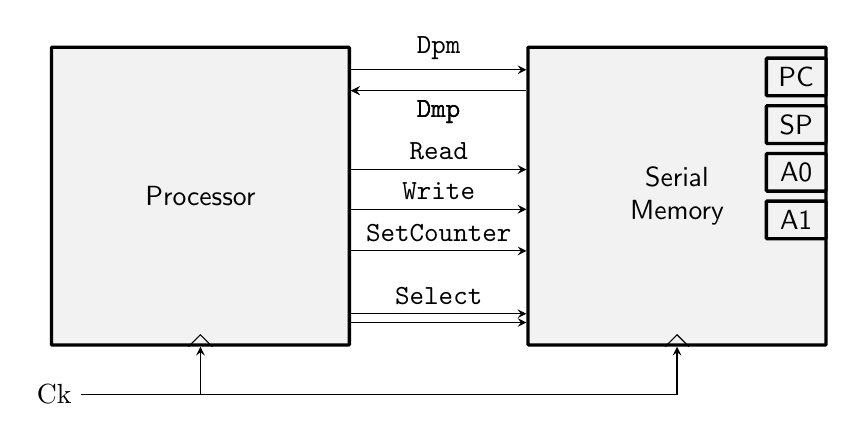
\begin{tikzpicture}
    \node[hwblock, minimum width=25ex,minimum height=25ex] (p) at (-10ex,0)  {Processor} ;
    \node[hwblock, minimum width=25ex,minimum height=25ex, align=center] (m) at (30ex,0)  {Serial\\ Memory} ;
    \node[hwblock,minimum height=3ex,minimum width=5ex] (pc) at (40ex,10ex)  {PC} ;
    \node[hwblock,minimum height=3ex,minimum width=5ex] (pc) at (40ex,6ex)  {SP} ;
    \node[hwblock,minimum height=3ex,minimum width=5ex] (pc) at (40ex,2ex)  {A0} ;
    \node[hwblock,minimum height=3ex,minimum width=5ex] (pc) at (40ex,-2ex)  {A1} ;
    \draw[hwwire,->] (p.40) -- (m.140) node[midway,above]{\texttt{Dpm}};
    \draw[hwwire,<-] (p.35) -- (m.145) node[midway,below]{\texttt{Dmp}};

    \draw[hwwire,->] (p.10) -- (m.170) node[midway,above]{\texttt{Read}};
    \draw[hwwire,->] (p.355) -- (m.185) node[midway,above]{\texttt{Write}};
    \draw[hwwire,->] (p.340) -- (m.200) node[midway,above]{\texttt{SetCounter}};
    \draw[hwwire,->] (p.322) -- (m.218) node[midway,above]{\texttt{Select}};
    \draw[hwwire,->] (p.320) -- (m.220) node[midway,above]{};
    \draw[hwwire,<-] (p.35) -- (m.145) node[midway,below]{\texttt{Dmp}};
    \draw[hwwire,<-] (m.south) -- ++(0,-4ex) -- ++(-50ex,0) node[left]{Ck};
    \draw[hwwire,<-] (p.south) -- ++(0,-4ex);
    \draw[hwwire,-] (p.south)  ++(-1ex, 0) -- ++(1ex,1ex) -- ++(1ex,-1ex); % horloge
    \draw[hwwire,-] (m.south)  ++(-1ex, 0) -- ++(1ex,1ex) -- ++(1ex,-1ex); % horloge
  \end{tikzpicture}
  \end{center}
\end{figure}


On a 4 compteurs d'adresses, chacun  répliqué dans le processeur et dans la mémoire (Table~\ref{tab:counters}).


Les instructions \texttt{readze}, \texttt{readse} et \texttt{write} lisent ou écrivent le nombre spécifié de bits tout en incrémentant les compteurs correspondant.

On peut émuler une instruction de lecture/écriture mémoire d'un processeur classique en deux instructions: un \texttt{setctr} puis un \texttt{readze} ou \texttt{readse} ou \texttt{write}.

Les instructions \texttt{push} et \texttt{pop} implémentent une pile descendante en mémoire: 
\begin{itemize}
\item \texttt{push} \emph{size} \emph{reg} réalise: \\
  $\mathit{sp}\leftarrow \mathit{sp}-\mathit{size}$\\ \texttt{setctr} \textit{sp}\\ \texttt{write}  \textit{sp} \textit{size} \textit{reg} \\   $\mathit{sp}\leftarrow \mathit{sp}-\mathit{size}$\\ \texttt{setctr} \textit{sp}
\item \texttt{pop} \emph{size} \emph{reg} est un raccourci offert par l'assembleur pour \\\texttt{readze} \textit{sp} \emph{size} \emph{reg}\\
  
\end{itemize}

\begin{table} 
  \caption{Counters. Ces deux bits sont transmis sur le signal \texttt{Select} de la figure~\ref{fig:overview}. }
  \label{tab:counters}
\begin{center}
  \begin{tabular}{|l|l|l|}
    \hline  
  encoding  & mnemonic & description \\
    \hline  
    \hline  
    00& \texttt{pc} &  program counter\\
    \hline
    01& \texttt{sp} & stack pointer\\
    \hline
    10& \texttt{a0} &  generic address counter\\
    \hline
    11& \texttt{a1} &  generic address counter\\
    \hline
  \end{tabular}
\end{center}
\end{table}

\section{Coût des opérations}
Le coût intéressant de cette étude est le nombre de bits échangé sur les fils de données. On distinguera trois types de données échangées : 
\begin{enumerate}
\item les instructions du programme (code lu par le processeur).
\item les données explicitement lues ou écrites (à l'aide de \texttt{readze}, par exemple)
\item Les bits d'adresses (typiquement, l'affectation de compteurs)
\end{enumerate}

Par exemple, \texttt{push 32 r0} fait d'abord transiter $7$ bits de la mémoire au processeur pour l'opérande, $3$ pour le registre. L'instruction est lue. Il faudra ensuite faire reculer le pointeur de pile de $32$ bits : $64$ bits pour récupérer \texttt{sp}, $64$ autres pour l'affecter. Les $32$ bits de \texttt{r0} sont écrits, puis on fait de nouveau reculer le pointeur de pile : $64$ bits. Soit un total d'instructions lues de $10$, $32$ bits de lus, et $192$ bits de compteurs.
La table \ref{tab:costs} résume le coût de chaque opération.

\subsection{Combien de registres ?}
Le nombre de registres est un compromis entre le nombre d'accès à la pile en mémoire et la taille des instructions : doubler le nombre de registres demande d'ajouter un sinon deux bits à presque toutes les instructions, avoir trop peu de registres oblige à utiliser fréquemment la pile. On peut {\it a priori} considérer que $4$ registres rend le processeur impraticable, et $16$ est sufisamment confortable pour programmer.\par
Avec huit registres, et pas mal d'astuce (par exemple, comment échanger deux registre sans utiliser de registre intermédiaire ?), les élèves s'en sont sortis avec des statistiques de \texttt{push} raisonnables (inférieures à 1\% des instructions). On peut donc espérer avec un \texttt{push} efficace un gain optimal avec seulement 8 registres. Cependant, la pénurie de registres restant d'actualité, on peut penser qu'un gain serait fait avec, par exemple une fenêtre de registres comme sur le SPARC.

\subsection{Bits de compteurs}
\subsubsection{choix initiaux}
On a fait le choix de ne pas faire d'adressage par registre : en effet, cela aurait coûté 64 bits d'adresse par adressage. Les compteurs permettent de faire autant avec seulement 2 bits à chaque adresse. En contrepartie, l'arithmétique sur les pointeurs devient extrêmement coûteuse : charger une adresse dans un registre ; faire une opération arithmétique ; affecter l'adresse avec le registre. Cependant, on espère que la plupart du temps, les données sont lues de manière séquencielle, et que donc un adressage avec post-incrément suffit à limiter l'arithmétique des pointeurs.\par
Cette affirmation est à relativiser : par exemple, le pc lit les données séquentiellement la plupart du temps. De même, dans les expériences, un écran avait été mappé sur la mémoire, et on pouvait l'effacer en écrivant plusieurs fois \texttt{0x0} à son adresse. Cependant, un contre-exemple très souvent utilisé est le \texttt{push}, qui nécessite un pré-decrément (le post-incrément oblige à affecter deux fois \texttt{sp}) ou encore la multiplication de matrices, gourmande en compteurs.
\subsubsection{améliorations}
La première amélioration, proposée dès le départ est de conserver une copie de chaque compteur dans le processeur. Ainsi, les échanges de bits de compteurs ne sont nécessaires que pour synchroniser les compteurs du processeur et de la mémoire : \texttt{getctr} ne coûte plus aucun bit de compteurs, on a aussi un gain sur le \texttt{push}
Ensuite, lors d'une affectation de compteurs, on n'est pas obligés d'écrire tous les bits s'ils sont envoyés poids faible d'abord. Si on envoie $n\leqslant 64$ bits à la mémoire, la mémoire peut écrire ces $n$ bits et remplire les $64-n$ autres avec des zéros. Cela diminuerait grandement le coût des affectations du pc, très proche du début de la mémoire (le code est stocké en \texttt{0x0}). Une autre idée, plus générale, serait de ne pas toucher aux $64-n$ derniers bits. On aurait un gain lors d'affectations proches en mémoire (même si bien sûr on ne peut rien garantir : \texttt{0x1000000 - 0x1 = 0xffffff})\par
Une autre amélioration, non-implémentée, serait d'ajouter des instructions d'incrémentation des compteurs par un registre ou une constante. On remplacerait les trois instructions \texttt{getctr a0 r0 ; add2 r0 r1 ; setctr a0 r0} par l'unique \texttt{incrctr a0 r0}. Si on ne gagne pas sur le nombre de bits de compteurs échangés (toujours $64$), cette instruction est assez facile à implanter en machine, on factorise un trio d'instruction assez présent dans la boucle interne de nombreux programmes (par exemple la multiplication matricielle) en une seule, et on gagne un registre.

\subsubsection{le problème de la pile}
Si avec le post-incrément, le \texttt{pull} ne coûte rien, dans la version naïve, le push est extrêmement coûteux : \texttt{push 32 r0} fait d'abord transiter $7$ bits de la mémoire au processeur pour l'opérande, $3$ pour le registre. L'instruction est lue. Il faudra ensuite faire reculer le pointeur de pile de $32$ bits : $64$ bits pour récupérer \texttt{sp}, $64$ autres pour l'affecter. Les $32$ bits de \texttt{r0} sont écrits, puis on fait de nouveau reculer le pointeur de pile : $64$ bits. Soit un total d'instructions lues de $10$, $32$ bits de lus, et $192$ bits de compteurs.\par
C'est un problème : comme on l'a vu l'efficacité du \texttt{push} détermine la quantité de registres nécessaires. La première amélioration proposée permet de faire descendre le coût du \texttt{push} à 128 bits, et plus si on décide d'un endroit adéquat pour placer le fond de la pile. Cependant, un gain énorme serait d'autoriser l'écriture avec pré-décrément : en écrivant les bits un à un à l'envers et en pré-décrément sur sp, on n'a plus besoin d'affecter sp. Le nombre de bits d'adresse dus au push retomberait à 0. Une manière assez simple de l'implémenter et de faire transiter le sens d'écriture sur le fil \texttt{Read} : 0 indiquerait post-incrément, et 1 pré-décrément. On pourrait même alors imaginer un \texttt{push} prenant en argument un compteur. Ainsi, chaque compteur pourrait devenir une pile.

\begin{table}[!h]
  \caption{Coûts des opérations}
  \label{tab:costs}
  On propose une première version naïve du coût de chaque opération, pour une architecture 64 bits. La taille d'une instruction étant variable, il faut à chaque fois l'ajouter dans les instructions lues.
  \begin{center}
  \begin{tabular}{|l|c|c|c|}
    \hline  
    type  & instructions lues & données lues/écrites & compteurs \\
    \hline  
    \hline
    \texttt{arith} \reg\ \reg\ &  $6$ & & \\
    \hline
    \texttt{arith} \reg\ \reg\ \reg\ & $9$ & & \\
    \hline
    \texttt{arith} \reg\ \const\ & $3$ + \const & & \\
    \hline
    \texttt{arith} \reg\ \reg\ \const\ & $6$ + \const & & \\
    \hline
    \texttt{r/w} \ctr\ \size\ \reg & $2$ + \size\ + $3$ & \size & \\
    \hline
    \texttt{get-,setctr} \ctr\ \reg\ & $2$ + $3$ & & $64$ \\
    \hline
    \texttt{jump} & \addr\ & & $64$ \\
    \hline
    \texttt{jumpif} \cond & $3$ + \addr\ & & $0$ ou $64$\\
    \hline
    \texttt{call} \addr & \addr\ & & $64$\\
    \hline
    \texttt{return} & & & $64$\\
    \hline
    \texttt{push} \size\ \reg & $3$ & \size & $192$\\
    \hline
  \end{tabular}
  \end{center}
Après améliorations, on arrive à ce nouveau tableau :
  \begin{center}
    \begin{tabular}{|l|c|c|c|}
      \hline  
      type  & instructions lues & données lues/écrites & compteurs \\
      \hline  
      \hline
      \texttt{getctr} \ctr\ \reg\ & $2$ + $3$ & & \\
      \hline
      \texttt{setctr} \ctr\ \reg\ & $2$ + $3$ & & $\leqslant 64$ \\
      \hline
      \texttt{jump} & \addr\ & & $\leqslant 64$ \\
      \hline
      \texttt{jumpif} \cond & $3$ + \addr\ & & $0$ ou $\leqslant 64$\\
      \hline
      \texttt{call} \addr & \addr\ & & $\leqslant 64$\\
      \hline
      \texttt{return} & & & $\leqslant64$\\
      \hline
      \texttt{push} \size\ \reg & $3$ & \size &\\
      \hline
    \end{tabular}
  \end{center}
\end{table}
  
\end{document}
